\documentclass[border=6pt]{standalone}
% Redrawn after Figure 1 of Radford et al., "Learning Transferable Visual Models
% From Natural Language Supervision", ICML 2021. The photographs in the original
% are replaced by placeholders.

% --- packages (mirror these in meta.json "requires") ---
\usepackage[T1]{fontenc}
\usepackage{mathptmx}
\usepackage[scaled=0.92]{helvet}
\usepackage{courier}
\renewcommand{\familydefault}{\sfdefault}
\usepackage{tikz}
\usetikzlibrary{arrows.meta}

% --- colors sampled from the original figure ---
\definecolor{cliptext}{HTML}{E1D5E7}
\definecolor{cliptextline}{HTML}{9673A6}
\definecolor{clipimage}{HTML}{D5E8D4}
\definecolor{clipimageline}{HTML}{82B366}
\definecolor{clipmatch}{HTML}{DAE8FC}
\definecolor{clipmatchline}{HTML}{6C8EBF}
\definecolor{clipcell}{HTML}{B3B3B3}
\definecolor{clipwire}{HTML}{4D4D4D}
\definecolor{clipclass}{HTML}{B5739D}
\definecolor{clipphoto}{HTML}{C9CDC4}
\definecolor{clipphotoshape}{HTML}{8E968A}

% ==== parameters (edit these) ============================================
\def\gridunit{0.0134}   % size of one layout unit (cm); scales the whole drawing
% labels
\def\stageonelabel{(1) Contrastive pre-training}
\def\stagetwolabel{(2) Create dataset classifier from label text}
\def\stagethreelabel{(3) Use for zero-shot prediction}
\def\textencoderlabel{Text\\Encoder}
\def\imageencoderlabel{Image\\Encoder}
\def\trainingtextlabel{Pepper the\\aussie pup}
\def\rowsym{I}   % image embedding symbol
\def\colsym{T}   % text embedding symbol
\def\lastindex{N}
\def\classa{plane}
\def\classb{car}
\def\classc{dog}
\def\classd{bird}
\def\classslotlabel{\{object\}}
\def\promptprefix{A photo of}
\def\promptjoin{a}
\def\predictedclass{dog}
% =========================================================================

\begin{document}
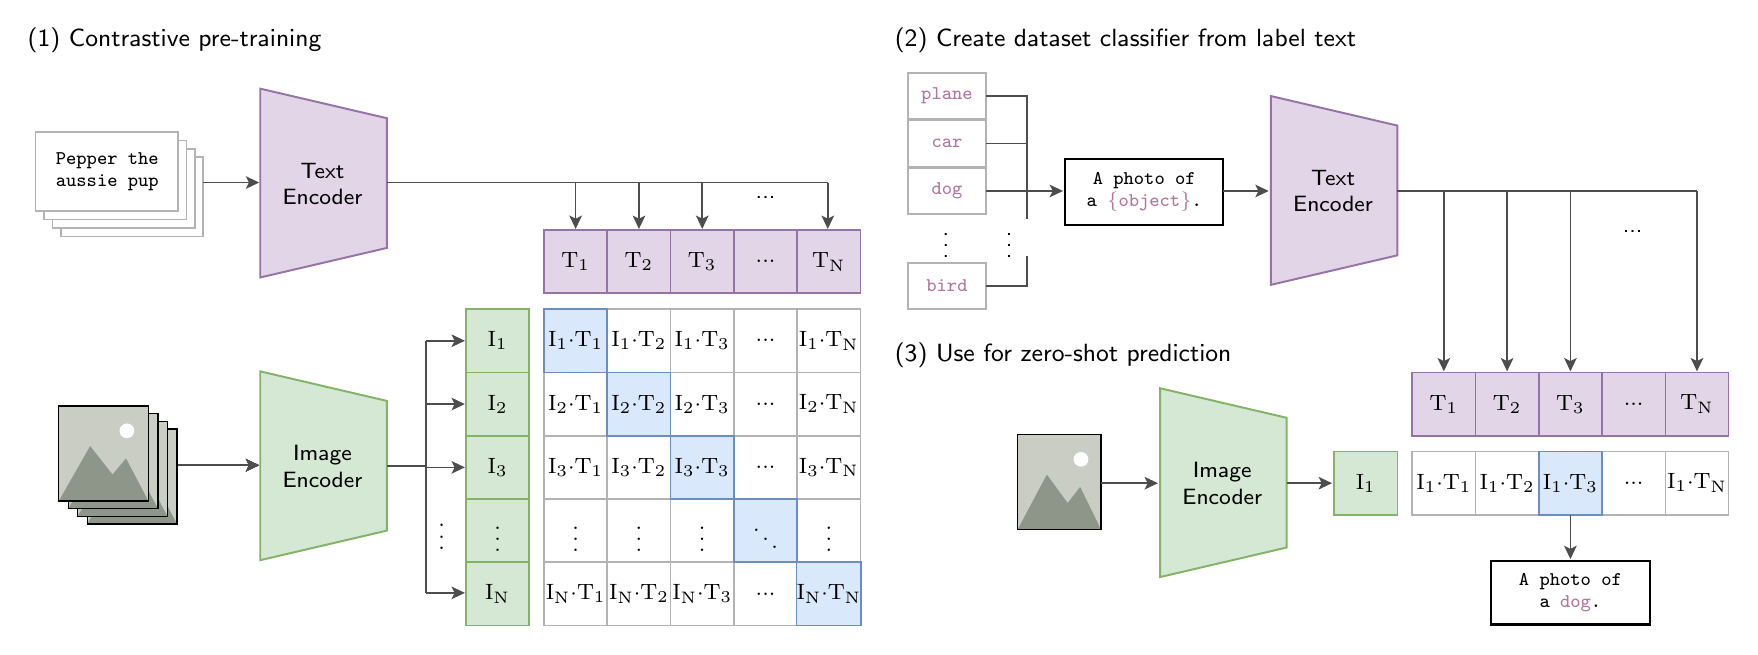
\begin{tikzpicture}[
    x=\gridunit cm, y=-\gridunit cm,
    >={Stealth[length=1.7mm, width=1.6mm, inset=0.4mm]},
    font=\footnotesize,
    wire/.style={draw=clipwire, line width=0.6pt},
    flow/.style={wire, ->},
    stage/.style={font=\small, anchor=west, inner sep=0pt},
    encoder text/.style={align=center, inner sep=0pt},
    sheet/.style={draw=clipcell, line width=0.6pt, fill=white},
    tt/.style={font=\scriptsize\ttfamily, align=center, inner sep=0pt},
    cell/.style={
      line width=0.6pt, inner sep=0pt, font=\footnotesize\rmfamily,
      minimum width=60*\gridunit cm, minimum height=60*\gridunit cm,
    },
    textcell/.style={cell, draw=cliptextline, fill=cliptext},
    imagecell/.style={cell, draw=clipimageline, fill=clipimage},
    scorecell/.style={cell, draw=clipcell, fill=white},
    matchcell/.style={cell, draw=clipmatchline, fill=clipmatch},
    black box/.style={draw=black, line width=0.75pt, fill=white, align=center, inner sep=0pt},
  ]
  % A trapezoid encoder: left x, top of its left edge, fill, stroke, label.
  \newcommand{\encoder}[5]{
    \draw[draw=#4, fill=#3, line width=0.7pt] (#1,#2) -- ++(120,28) -- ++(0,123) -- ++(-120,28) -- cycle;
    \node[encoder text] at (#1+59,#2+90) {#5};
  }
  % Placeholder for a photograph: x0, y0, x1, y1. Replace it with \includegraphics.
  \newcommand{\photo}[4]{
    \pgfmathsetmacro\pxa{#1}\pgfmathsetmacro\pya{#2}\pgfmathsetmacro\pxb{#3}\pgfmathsetmacro\pyb{#4}
    \begin{scope}
      \clip (\pxa,\pya) rectangle (\pxb,\pyb);
      \fill[clipphoto] (\pxa,\pya) rectangle (\pxb,\pyb);
      \fill[clipphotoshape] (\pxa,\pyb) -- ({\pxa+(\pxb-\pxa)*0.35},{\pya+(\pyb-\pya)*0.42})
        -- ({\pxa+(\pxb-\pxa)*0.6},{\pya+(\pyb-\pya)*0.72}) -- ({\pxa+(\pxb-\pxa)*0.75},{\pya+(\pyb-\pya)*0.55})
        -- (\pxb,\pyb) -- cycle;
      \fill[white] ({\pxa+(\pxb-\pxa)*0.76},{\pya+(\pyb-\pya)*0.26}) ellipse [x radius=7, y radius=7];
    \end{scope}
    \draw[black, line width=0.5pt] (\pxa,\pya) rectangle (\pxb,\pyb);
  }
  \newcommand{\pair}[2]{\rowsym$_{\mathrm{#1}}{\cdot}$\colsym$_{\mathrm{#2}}$}

  % =================== (1) contrastive pre-training =====================
  \node[stage] at (20,25) {\stageonelabel};

  % --- text branch ---
  \foreach \d in {24,16,8,0} \draw[sheet] (28+\d,112+\d) rectangle ++(135,75);
  \node[tt] (train-text) at (96,150) {\trainingtextlabel};
  \draw[flow] (187,160) -- (240,160);
  \encoder{241}{71}{cliptext}{cliptextline}{\textencoderlabel}
  \draw[wire] (361,160) -- (779,160);
  \foreach \x in {540,600,660,779} \draw[flow] (\x,160) -- (\x,204);
  \node at (720,174) {...};
  \foreach \j/\lab in {1/1,2/2,3/3,5/\lastindex} \node[textcell] (train-t\j) at (480+60*\j,235) {\colsym$_{\mathrm{\lab}}$};
  \node[textcell] (train-t4) at (720,235) {...};

  % --- image branch ---
  \foreach \d in {27,18,9,0} \photo{50+\d}{372+\d*0.8}{135+\d}{462+\d*0.8}
  \draw[flow] (163,428) -- (240,428);
  \encoder{241}{339}{clipimage}{clipimageline}{\imageencoderlabel}
  \draw[wire] (361,429) -- (398,429);
  \draw[wire] (398,310) -- (398,549);
  \foreach \y in {310,370,430,549} \draw[flow] (398,\y) -- (435,\y);
  \node[font=\footnotesize\rmfamily] at (413,488) {$\vdots$};
  \foreach \i/\lab in {1/1,2/2,3/3,5/\lastindex} \node[imagecell] (train-i\i) at (466,250+60*\i) {\rowsym$_{\mathrm{\lab}}$};
  \node[imagecell] (train-i4) at (466,490) {$\vdots$};

  % --- similarity matrix; the diagonal is drawn last so its border stays visible ---
  \foreach \i/\il in {1/1,2/2,3/3,5/\lastindex} {
    \foreach \j/\jl in {1/1,2/2,3/3,5/\lastindex} {
      \ifnum\i=\j\else \node[scorecell] (m-\i-\j) at (480+60*\j,250+60*\i) {\pair{\il}{\jl}}; \fi
    }
    \node[scorecell] (m-\i-4) at (720,250+60*\i) {...};
    \node[scorecell] (m-4-\i) at (480+60*\i,490) {$\vdots$};
  }
  \foreach \i/\il in {1/1,2/2,3/3,5/\lastindex} \node[matchcell] (m-\i-\i) at (480+60*\i,250+60*\i) {\pair{\il}{\il}};
  \node[matchcell] (m-4-4) at (720,490) {$\ddots$};

  \begin{scope}[xshift=810*\gridunit cm]
  % =================== (2) classifier from label text ===================
  \node[stage] at (32,25) {\stagetwolabel};
  \foreach \lab/\top in {\classa/56,\classb/101,\classc/146,\classd/236} {
    \draw[sheet] (45,\top) rectangle ++(74,44);
    \node[tt, text=clipclass] at (82,\top+22) {\lab};
  }
  \node at (81,212) {$\vdots$};
  \node at (141,212) {$\vdots$};
  \draw[wire] (119,78) -- (158,78) -- (158,195);
  \draw[wire] (119,123) -- (158,123);
  \draw[wire] (158,230) -- (158,258) -- (119,258);
  \draw[flow] (119,168) -- (192,168);
  \node[black box, tt, minimum width=150*\gridunit cm, minimum height=62*\gridunit cm] (prompt) at (269,169)
    {\promptprefix\\\promptjoin\ \textcolor{clipclass}{\classslotlabel}.};
  \draw[flow] (344,168) -- (387,168);
  \encoder{389}{78}{cliptext}{cliptextline}{\textencoderlabel}
  \draw[wire] (509,168) -- (793,168);
  \foreach \x in {553,613,673,793} \draw[flow] (\x,168) -- (\x,339);
  \node at (732,206) {...};
  \foreach \j/\lab in {1/1,2/2,3/3,5/\lastindex} \node[textcell] (test-t\j) at (493+60*\j,370) {\colsym$_{\mathrm{\lab}}$};
  \node[textcell] (test-t4) at (733,370) {...};

  % =================== (3) zero-shot prediction =========================
  \node[stage] at (32,324) {\stagethreelabel};
  \photo{149}{399}{228}{489}
  \draw[flow] (228,445) -- (282,445);
  \encoder{284}{355}{clipimage}{clipimageline}{\imageencoderlabel}
  \draw[flow] (404,445) -- (447,445);
  \node[imagecell] (test-i1) at (479,445) {\rowsym$_{\mathrm{1}}$};
  \foreach \j/\lab in {1/1,2/2,5/\lastindex} \node[scorecell] (score-\j) at (493+60*\j,445) {\pair{1}{\lab}};
  \node[scorecell] (score-4) at (733,445) {...};
  \node[matchcell] (score-3) at (673,445) {\pair{1}{3}};
  \draw[flow] (673,475) -- (673,517);
  \node[black box, tt, minimum width=150*\gridunit cm, minimum height=60*\gridunit cm] (answer) at (673,549)
    {\promptprefix\\\promptjoin\ \textcolor{clipclass}{\predictedclass}.};
  \end{scope}

\end{tikzpicture}
\end{document}
